%%%%%%%%%%%%%%%%%%%%%%%%%%%%%%%%%%%%%%%%%%%%%%%%%%%%%%%%%%%%%%%%%%%%%%%%%%%%%%
% Template LaTeX Template Version 1.0 (December 8 2014)
%
% This template has been downloaded from: http://www.LaTeXTemplates.com
%
% Original author: Brandon Fryslie With extensive modifications by: Vel
% (vel@latextemplates.com)
%
% License: CC BY-NC-SA 3.0 (http://creativecommons.org/licenses/by-nc-sa/3.0/)
%
% Authors: Sabbir Ahmed
% 
%%%%%%%%%%%%%%%%%%%%%%%%%%%%%%%%%%%%%%%%%%%%%%%%%%%%%%%%%%%%%%%%%%%%%%%%%%%%%%

\documentclass[paper=usletter, fontsize=12pt]{article}
%%%%%%%%%%%%%%%%%%%%%%%%%%%%%%%%%%%%%%%%%
% Contract Structural Definitions File Version 1.0 (December 8 2014)
%
% Created by: Vel (vel@latextemplates.com)
% 
% This file has been downloaded from: http://www.LaTeXTemplates.com
%
% License: CC BY-NC-SA 3.0 (http://creativecommons.org/licenses/by-nc-sa/3.0/)
%
%%%%%%%%%%%%%%%%%%%%%%%%%%%%%%%%%%%%%%%%%

\usepackage{geometry} % Required to modify the page layout
\usepackage{multicol}
\usepackage{amsmath}
\usepackage{amssymb}

\usepackage[pdftex]{graphicx}
\usepackage{wrapfig}
\usepackage[font=scriptsize, labelfont=bf]{caption}
\usepackage[utf8]{inputenc} % Required for including letters with accents
\usepackage[T1]{fontenc} % Use 8-bit encoding that has 256 glyphs

\usepackage{avant} % Use the Avantgarde font for headings
\usepackage{courier}
\usepackage{xparse}
\usepackage{xcolor}
\usepackage{listings}  % for code verbatim and console outputs

\setlength{\textwidth}{16cm} % Width of the text on the page
\setlength{\textheight}{23cm} % Height of the text on the page
\setlength{\oddsidemargin}{0cm} % Width of the margin - negative to move text left, positive to move it right
\setlength{\topmargin}{-1.25cm} % Reduce the top margin

\setlength{\parindent}{0mm} % Don't indent paragraphs
\setlength{\parskip}{2.5mm} % Whitespace between paragraphs
\renewcommand{\baselinestretch}{1.5}

\definecolor{green}{rgb}{0.18, 0.55, 0.34}

\graphicspath{ {figures/} }
\captionsetup[table]{skip=10pt}

\lstset{language=C, keywordstyle={\bfseries \color{black}}}

% defines algorithm counter for chapter-level
\newcounter{nalg}[section]

%defines appearance of the algorithm counter
\renewcommand{\thenalg}{\thesection .\arabic{nalg}}

% defines a new caption label as Algorithm x.y
\DeclareCaptionLabelFormat{algocaption}{Algorithm \thenalg}

% defines the algorithm listing environment
\lstnewenvironment{pseudocode}[1][] {
    \refstepcounter{nalg}  % increments algorithm number
    \captionsetup{font=normalsize, labelformat=algocaption, labelsep=colon}
    \lstset{
        breaklines=true,
        mathescape=true,
        numbers=left,
        numberstyle=\scriptsize,
        basicstyle=\footnotesize\ttfamily,
        keywordstyle=\color{black}\bfseries,
        keywords={input, output, return, parallel, function, for, to, in, if,
        else, foreach, while, and, or, new, print},
        xleftmargin=.04\textwidth,
        #1
    }
}{}

\renewcommand{\familydefault}{\sfdefault}  % default font for entire document
 % specifies the document layout and style

\begin{document}

    \documentinfo {\textbf{Homework 7: VGA Circle Report}}
    {\today} {Sabbir Ahmed}
    \vspace{-0.1in}

    \section{Background} In this project students will explicitly implement a
    computational finite-state machine, utilize rescheduling and resource
    sharing, and become familiar with the concept of using an on-chip clock
    multiplier. Students will leverage the faster clock to implement
    computations in a serial fashion. In this HW students will display a circle
    on the screen, examine analysis reports, and modify synthesis options.

    \section{Design Approach} The source code for interfacing with UART was
    provided. The controller FSM was implemented to provide all the glue logic
    required to interface the UART with the \texttt{sqrt} module and the block
    RAM. The multiplexer controlling the \texttt{tx\_data} in the datapath is
    integrated into the controller module as the states \texttt{ramhi} and
    \texttt{ramlo}. Figure \ref{fig:block} provides the top-level block diagram
    of the project implementation.

        \begin{figure}[ht]
            \begin{center}
                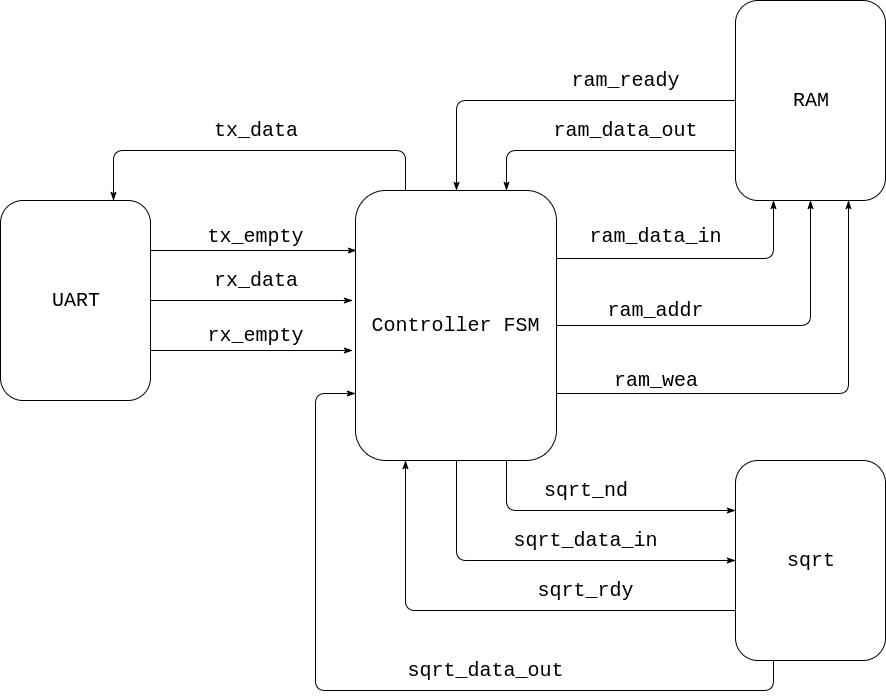
\includegraphics[width=1\textwidth]{block_diagram.png}
                \caption{Block Diagram of the Implementation}
                \label{fig:block}
            \end{center}
        \end{figure}

        \subsection{Controller FSM} The controller FSM consists of 7 states
        visualized in Figure \ref{fig:states}.

            \begin{figure}[ht]
                \begin{center}
                    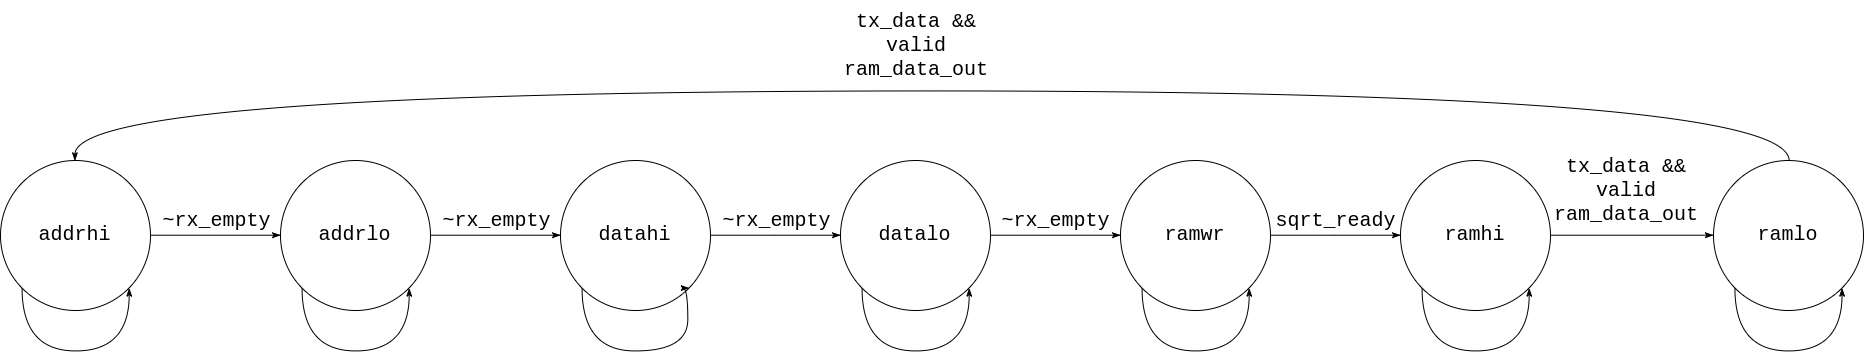
\includegraphics[width=1\textwidth]{state_diagram.png}
                    \caption{State Diagram of the Implementation of the
                    Controller}
                    \label{fig:states}
                \end{center}
            \end{figure}

            \subsubsection{addrhi} This is the initial state of the controller
            to detect when the high bytes of the RAM block address from
            \texttt{rx\_data} have been transferred from the UART. The state
            proceeds to \texttt{addrlo} when the shifter at \texttt{rx} is
            empty and \texttt{AH} is ready.

            \subsubsection{addrlo} Activated when the shifter at \texttt{rx} is
            empty and \texttt{AH} is ready. This is the second state of the
            controller to detect when the low bytes of the RAM block address
            from \texttt{rx\_data} have been transferred from the UART. The
            state saves the entire 12-bit address of the RAM block and then
            proceeds to \texttt{datahi} when the shifter at \texttt{rx} is
            empty and \texttt{AL} is ready.

            \subsubsection{datahi} Activated when the shifter at \texttt{rx} is
            empty and \texttt{AL} is ready. This is the third state of the
            controller to detect when the high bytes of the RAM block input
            data from \texttt{rx\_data} have been transferred from the UART.
            The state proceeds to \texttt{datahi} when the shifter at
            \texttt{rx} is empty and \texttt{DH} is ready.

            \subsubsection{datalo} Activated when the shifter at \texttt{rx} is
            empty and \texttt{DH} is ready. This is the fourth state of the
            controller to detect when the low bytes of the RAM block input data
            from \texttt{rx\_data} have been transferred from the UART. The
            state sends the entire 16-bit data to the \texttt{sqrt} module and
            then proceeds to \texttt{ramwr} when the shifter at \texttt{rx} is
            empty and \texttt{DL} is ready.

            \subsubsection{ramwr} Activated when the \texttt{sqrt} module is
            and \texttt{DL} is ready. This is the fifth state of the controller
            to write to the RAM block. The state sends the entire 12-bit
            address and the output of the \texttt{sqrt} module to the RAM block
            and then proceeds to \texttt{ramhi}.

            \subsubsection{ramhi} Activated when the shifter at \texttt{tx} is
            empty and data read from the RAM block is valid and ready. This is
            the sixth state of the controller to read from the RAM block with
            the same address and passed back to the UART. The state sends the
            high 8-bit data read from the \texttt{sqrt} module to the
            \texttt{tx\_data} in the UART.

            \subsubsection{ramlo} Activated when the shifter at \texttt{tx} is
            empty and data read from the RAM block is valid and ready. This is
            the final state of the controller to read from the RAM block with
            the same address and passed back to the UART. The state sends the
            low 8-bit data read from the \texttt{sqrt} module to the
            \texttt{tx\_data} in the UART.

    \newpage
    \section{Testing} The project submission includes test benches for the
    controller as well as the top-level module integrating all the modules.
    Figure \ref{fig:tbwav} shows an example use of the implementation with the
    memory file contents: 01, 01, 00, 04.

    \begin{figure}[ht]
        \begin{center}
            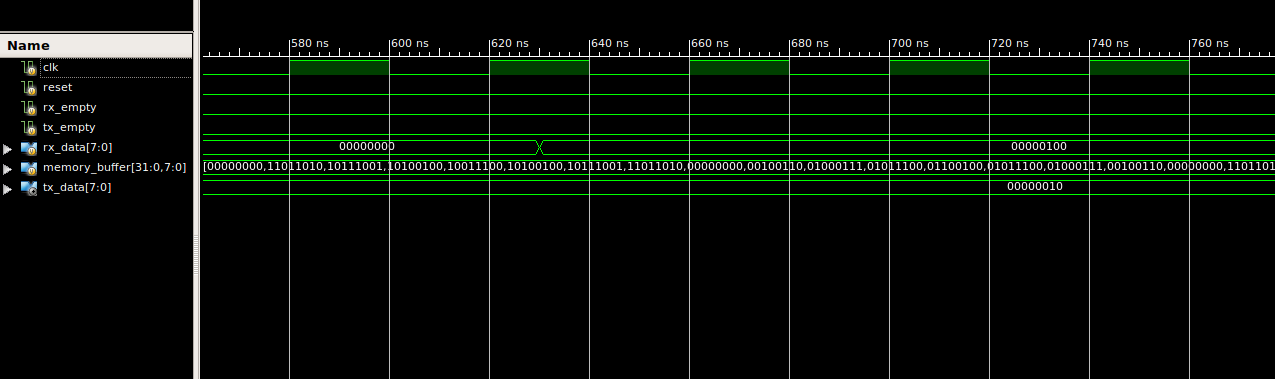
\includegraphics[width=1\textwidth]{controller_tb_wav.png}
            \caption{Sample Testbench Waveform of the Controller Module}
            \label{fig:tbwav}
        \end{center}
    \end{figure}

    Figure \ref{fig:tbwav} demonstrates the unit after its final state. The
    address to the RAM block was passed as 0001 0000 0001 (low 4 bits of the
    high 01 hex value and the entire low 01 hex value). The data passed to the
    \texttt{sqrt} module was 0000 0000 0000 0100 (00 and 04). The \texttt{sqrt}
    module returns 0000 0010 ($\sqrt{\text{4}}=\text{2}$).

\end{document}
